\subsubsection*{Т20}


Для следующих четырёх гамильтоновых систем оценим меру устойчивых, или неустойчивых траекторий к возмущениям $\varepsilon H_1$ при малых $(0 < \varepsilon \ll 1)$. Также построим графики линий уровня $H_0 (I_1, I_2)$ и отложим на них $\omega \colon  \omega_2 = \const$. 


\textbf{Первый случай}. Для гамильтониана и возмущения
\begin{equation*}
    H_0 = 42 I_1^2 + I_1 I_2 + 42 I_2^2, \hspace{5 mm} H_1 = 2 I_1 \sin(3 \varphi_1 - 18 \varphi_2),
\end{equation*}
можем перейти к переменным $\vc{J}, \ \vc{\psi}$ через производящую функцию вида
\begin{equation*}
    S + \vc{I} \cdot \vc{\varphi} + \varepsilon \frac{18}{5} \frac{2I_1}{84 I_1 + I_2} \cos(3 \varphi_1 - 18 \varphi_2),
\end{equation*}
к гамильтониану $\hat{H} = H_0(J_1, J_2)$, и, соотвественно ограниченными $I_1$, $I_2$. 

Система с $H_0$ является невырожденной 
\begin{equation*}
    \bigg| \frac{\partial^2 H}{\partial I_i \partial I_j} \bigg| = 
    \begin{pmatrix}
        84 & 1  \\
        1 & 84  \\
    \end{pmatrix} \neq 0,
\end{equation*}
а также изоэнергетически невырожденной
\begin{equation*}
     \det \begin{bmatrix}
        \vphantom{\dfrac{1}{2}}
            \dfrac{\partial^2 H_0}{\partial \vc{I}\T \partial \vc{I}} & \vc{\omega} \\
        \vphantom{\dfrac{1}{2}}
            \vc{\omega}\T & 0
        \end{bmatrix} = \begin{pmatrix}
            84 & 1 & 84 I_1 + I_2 \\
            1 & 84 & 84 I_2 + I_1 \\
            84 I_1 + I_2 & 84 I_2 + I_1 & 0 \\
        \end{pmatrix} = 14110 (42 I_1^2 + I_1 I_2 + 42 I_2^2) \sim H_0 > 0.
\end{equation*}
Таким образом мера траекторий, неустойчивых к возмущениям, равна нуля (а вообще выше мы показали, что их здесь нет).

\begin{figure}[h]
    \centering
    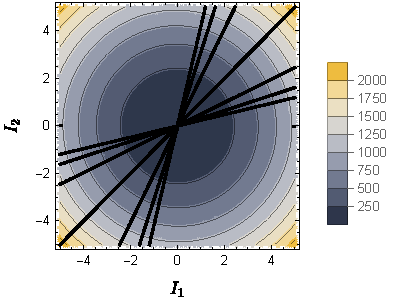
\includegraphics[width=0.4\textwidth]{figures/H1.pdf}
    \hspace{10 mm} 
    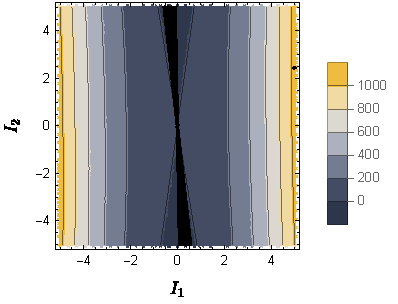
\includegraphics[width=0.4\textwidth]{figures/H2.pdf}
    \caption{Линии уровня для первого и второго случая.}
\end{figure}

Если посмотреть на
\begin{equation*}
    \frac{\omega_1}{\omega_2} = \frac{84 I_1 + I_2}{I_1 + 84 I_2} \in \mathbb{Q},
\end{equation*}
то можно заметить, что это просто линии, пересекающие центр графика $I_1(I_2)$ (нулевой меры). 



\textbf{Второй случай.} Для гамильтониана и возмущения
\begin{equation*}
    H_0 = 42 I_1^2 + I_1 I_2 - I_2^2,
    \hspace{5 mm} 
    H_1 = 3 I_2 \cos(2 \varphi_1 + 14 \varphi_2),
\end{equation*}
оценим меру неустойчивых траекторий. 

Система с $H_0$ невырожденна
\begin{equation*}
    \bigg| \frac{\partial^2 H}{\partial I_i \partial I_j} \bigg| = \det \begin{pmatrix}
        84 & 1  \\
        1 & -2  \\
    \end{pmatrix} = - 169 \neq 0,
\end{equation*}
также она при почти всех начальных условиях изоэнергетически невырожденна:
\begin{equation*}
         \det \begin{bmatrix}
        \vphantom{\dfrac{1}{2}}
            \dfrac{\partial^2 H_0}{\partial \vc{I}\T \partial \vc{I}} & \vc{\omega} \\
        \vphantom{\dfrac{1}{2}}
            \vc{\omega}\T & 0
        \end{bmatrix}  = 338 (7 I_1 - I_2)(6 I_1 + I_2),
\end{equation*}
но вырожденна при $7 I_1 = I_2$. В общем по КАМ-теории мера разрушившихся торов -- нуль.

Уравнения движения системы после возмущения:
\begin{align*}
    \dot{I}_1 &= - \partial_{\varphi_1} H = \varepsilon \cdot 6 I_2 \sin(2 \varphi_1 + 14 \varphi_2)\\ 
    \dot{I}_2 &= - \partial_{\varphi_2} H = \varepsilon \cdot 42 I_2 \sin(2 \varphi_1 + 14 \varphi_2)\\ 
    \dot{\varphi}_1 &= \partial_{I_1} H = 2 \cdot 42 I_1 + I_2 \\
    \dot{\varphi}_2 &= \partial_{I_2} H =I_1 - 2 I_2 + \varepsilon \cdot 3 \cos (2 \varphi_1 + 14 \varphi_2).
\end{align*}
Внимательно на это посмотрев можно заметить удачно выбранные числа:
\begin{equation*}
    \gamma \overset{\mathrm{def}}{=}  2 \varphi_1 + 14 \varphi_2,
    \hspace{5 mm} 
    \dot{\gamma} = 13 \cdot 2 (7 I_1 - I_2) + \varepsilon \cdot 3 \cos (\gamma).
\end{equation*}
Ещё более внимательный взгляд подскажет, что
\begin{equation*}
    \textstyle \frac{d }{d t} (7 I_1 - I_2) = 0,
\end{equation*}
таким образом при н.у. вида $I_1(0)= \frac{1}{7} I_0 (0)$ даст $7 I_1 - I_2 = 0$ $\forall t$. Тогда и $\dot{\gamma} = \varepsilon \cdot 3 \cos \gamma$, откуда
\begin{equation*}
    \tg \frac{\gamma}{2} = \frac{e^{3 \varepsilon t}-1}{e^{3 \varepsilon t}+1},
    \hspace{5 mm} 
    \lim_{t \to \infty} \tg \frac{\gamma}{2} = 1,
    \hspace{0.5cm} \Rightarrow \hspace{0.5cm}
    \gamma \underset{t \to \infty}{\to} \frac{\pi}{2}.
\end{equation*}
В таком случае в выражении для $\dot{I}_2$ $\sin \gamma \to 1$, тогда и
\begin{equation*}
    \dot{I}_2 = \varepsilon \cdot 42 I_2,
    \hspace{0.5cm} \Rightarrow \hspace{0.5cm}
    I_2 = \exp(\varepsilon \cdot 42 t), 
\end{equation*}
что неограниченно растёт, и траектория убегает.


Также была вырожденность с н.у. $I_1 (0) = - \frac{1}{6} I_2 (0)$, но $\frac{\omega_1}{\omega_2}$ подобраны не под эту скобку, и в решение там тор не ломается, решение периодично.


Здесь отношение частот аналогично первому случаю представляет
\begin{equation*}
    \frac{\omega_1}{\omega_2} = \frac{84 I_1 + I_2}{I_1 - 2 I_2} \in \mathbb{Q}
\end{equation*}
набор, проходящих через центр прямых, нулевой меры. 


\textbf{Третий случай.} Для гамильтониана и возмущения
\begin{equation*}
    H_0 = 36 I_1^2 + 12 I_1 I_2 + I_2^2,
    \hspace{5 mm} 
    H_1 = \left(42 I_1^2 + 13 I_1 I_2 + I_2^2\right) \cdot \cos^3(\varphi_1-6 \varphi_2),
\end{equation*}
оценим меру неустойчивых траекторий. 

\begin{figure}[h]
    \centering
    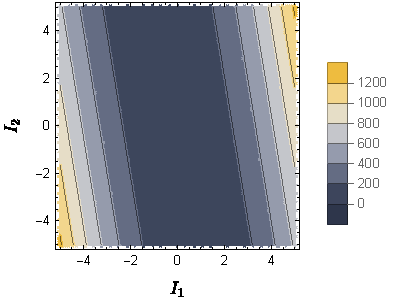
\includegraphics[width=0.4\textwidth]{figures/H3.pdf}
    \hspace{10 mm} 
    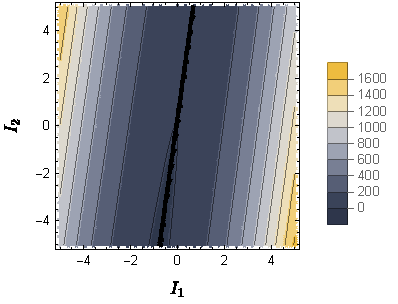
\includegraphics[width=0.4\textwidth]{figures/H4.pdf}
    \caption{Линии уровня для третьего и четвертого случая.}
\end{figure}



В этом случае система вырождена
\begin{equation*}
        \bigg| \frac{\partial^2 H}{\partial I_i \partial I_j} \bigg| = 0,
\end{equation*}
и изоэнергетически вырожденна:
\begin{equation*}
         \det \begin{bmatrix}
        \vphantom{\dfrac{1}{2}}
            \dfrac{\partial^2 H_0}{\partial \vc{I}\T \partial \vc{I}} & \vc{\omega} \\
        \vphantom{\dfrac{1}{2}}
            \vc{\omega}\T & 0
        \end{bmatrix}  = 0.
\end{equation*}
Далее покажем, что все траектории уходят в $\infty$.


Итак, уравнения движения
\begin{align*}
    \dot{I}_1 &= \varepsilon \left(
        42 I_1^2 + 13 I_1 I_2 + I_2^2
    \right) \cdot 3 \cos^2(\varphi_1-6\varphi_2) \sin(\varphi_1-6 \varphi_2), \\
    \dot{I}_2 &= \varepsilon\left(
        42 I_1^2 + 3 I_1 I_2 +I_2^2
    \right) \cdot 3 \cos^2 (\varphi_1 - 6 \varphi_2) \cdot 6 \sin(6 \varphi_2 -\varphi_1), \\
    \dot{\varphi}_1 &= 12 (6 I_1 + I_2) +  \varepsilon \cdot (42 \cdot 2 I_1 + 13 I_2) \cos^3(\varphi_1 - 6 \varphi_2), \\
    \dot{\varphi}_2 &= 2 (6 I_1 + I_2) + \varepsilon (13 I_1 +  2 I_2) \cos^3 (\varphi_1 - 6 \varphi_2).
\end{align*}
И снова удачно подобраны цифры:
\begin{equation*}
    \gamma \overset{\mathrm{def}}{=}  \varphi_1 - 6 \varphi_2 ,
    \hspace{5 mm} 
    \dot{\gamma} = \varepsilon \left[
        6 I_1 + I_2
    \right] \cdot \cos^3\left(
        \varphi_1 - 6 \varphi_2
    \right).
\end{equation*}
Удивительно так совпало, что множитель -- константа, 
\begin{equation*}
    6 \dot{I}_1 + \dot{I}_2 = 0, \ \Rightarrow \ 6 I_1 + I_2 = \theta = \const,
\end{equation*}
в новых обозначениях мы приходим к системе вида
\begin{equation*}
    \dot{\gamma} = \varepsilon \theta \cos^3(\gamma),
    \hspace{0.5cm} \Rightarrow \hspace{0.5cm}
    \frac{d \gamma}{d \cos^3 \gamma}  = \varepsilon \theta \d t.
\end{equation*}
Считая $7 I_1 + I_2 = \varkappa$, заметим, что
\begin{equation*}
    H_0 = \theta \varkappa, \hspace{5 mm} \dot{\kappa} = 3 \varkappa \cdot \varepsilon \theta \cos^2 (\gamma) \sin (\gamma).
\end{equation*}

Теперь можно пойти разными путями -- выберем наиболее универсальный:
\begin{equation*}
\frac{d \gamma}{d \cos^3 \gamma}  = \varepsilon \theta \d t,
\hspace{0.5cm} \Rightarrow \hspace{0.5cm}
    \exp\left(\frac{\sin \gamma}{\cos^2 \gamma}\right) \frac{1 + \tg \gamma/2}{1-\tg \gamma/2} = \exp\left( 2 \varepsilon \theta t\right).
\end{equation*}
И это замечательно, ведь получается, что при росте времени, $\gamma \to \pi/2$, а тогда выражение перепишется в виде ($\gamma = \pi/2-T$)
\begin{equation*}
    e^{1/T^2} \frac{2}{T} = \exp\left(
        \ln 2 - \ln T + \frac{1}{T^2}
    \right) = \exp(2 \varepsilon \theta t),
    \hspace{0.5cm} \Rightarrow \hspace{0.5cm}
    T^2 = \frac{1}{2\varepsilon \theta t},
\end{equation*}
где было учтено, что $\lim_{T\to 0} (1 - T^2 \ln T) = 1$. Этот замечательный результат можем подставить в $\dot{\varkappa}$:
\begin{equation*}
    \dot{\varkappa} \approx (3 \varepsilon \theta) \varkappa T^2,
    \hspace{0.5cm} \Rightarrow \hspace{0.5cm}
    \frac{d \varkappa}{\varkappa} = \frac{3}{2} \frac{d t}{d t},
    \hspace{0.5cm} \Rightarrow \hspace{0.5cm}
    \varkappa = C \cdot t^{3/2},
\end{equation*}
другими словами неограниченно растёт, что верно для всех траекторий, с ненулевым $\theta$. Таким образом мера неразрушившихся торов равна нулю. 

Здесь, так как система вырождена, отношение частот зафиксировано:
\begin{equation*}
    \frac{\omega_1}{\omega_2} = 6 \frac{12 I_1 + 2 I_2}{12I_1 + 2 I_2} = 6,
\end{equation*}
почти всюду. 





\textbf{Четвёртый случай}. Для гамильтониана и возмущения
\begin{equation*}
    H_0 = 49 I_1^2 - 14 I_1 I_2 + I_1^2 + 6 I_1 + I_2,
    \hspace{5 mm} 
    H_1 = 4 I_2 \sin^3 (3 \varphi_1 +  21 \varphi_2),
\end{equation*}
оценим меру неустойчивых траекторий. 

В этом случае система вырождена
\begin{equation*}
        \bigg| \frac{\partial^2 H}{\partial I_i \partial I_j} \bigg| = 0,
\end{equation*}
но при этом изоэнергетически невырожденна:
\begin{equation*}
         \det \begin{bmatrix}
        \vphantom{\dfrac{1}{2}}
            \dfrac{\partial^2 H_0}{\partial \vc{I}\T \partial \vc{I}} & \vc{\omega} \\
        \vphantom{\dfrac{1}{2}}
            \vc{\omega}\T & 0
        \end{bmatrix}  = -338.
\end{equation*}

Покажем, что для такой системы мера <<неустойчивых>> траекторий равна нулю. Уравнения движения такой возмущенной системы
\begin{align*}
    \dot{I}_1 &= - 36 I_2  \cdot \varepsilon \cos(3 \varphi_1 + 21 \varphi_2) \sin^2 (3 \varphi_1 + 21 \varphi_2), \\
    \dot{I}_2 &= - e` \cdot 12 \cdot 21 I_2 \cos(3 \varphi_1 + 21 \varphi_2) \sin^2 (3 \varphi_1 + 21 \varphi_2), \\
    \dot{\varphi}_1 &= 6 + 98 I_1 - 14, \\
    \dot{\varphi}_2 &= 1 - 14 I_1 + 2 I_2 + 4 \varepsilon \sin^3 (3 \varphi_1 + 21 \varphi_2).
\end{align*}
Собственные частоты системы:
\begin{equation*}
    \left\{\begin{aligned}
        \omega_1 &= 6 + 14(7 I_1 - I_2) \\
        \omega_2 &= 1 - 2 (7I_1-I_2).
    \end{aligned}\right.
\end{equation*}
Тогда и улетающие куда-то траектории должны иметь похожего вида силы (по идее), однако, получается, для этого должно выполняться соотношение
\begin{equation*}
    \omega_1 + 7 \omega_2 = 13,
\end{equation*}
и, хотя диофантовые уравнения решаются плохо, подставить в качестве частот $\omega_1 = \pm\{3, 9\}$ и $\omega_2 = \pm \{21, 63\}$ мы можем. Ни одна из пар $\{\omega_1, \omega_2\}$ не подходит, так что, по идее, мера резонансных торов равна нулю. 

У системы 
\begin{equation*}
    \frac{\omega_1}{\omega_2} = \frac{6 + 98 I_1 - 14 I_2}{1-14 I_1 + 2 I_2} = C \in \mathbb{Q}
\end{equation*}
 зависимость, как видно вырожденная:
 \begin{equation*}
     I_2 = \frac{C-6}{2(7+C)} + 7 I_1, 
 \end{equation*}
 для $\omega_2/\omega_1 = C$, таким образом все прямые такого вида отличаются параллельным переносом.